\documentclass[12pt, fleqn]{article}

\usepackage[left=0.75in, right=0.75in, bottom=0.75in, top=1.0in]{geometry}
\usepackage{amsmath}
\usepackage{amssymb}
\usepackage{amsthm}
\usepackage{mathtools}
\usepackage{hyperref}
\usepackage{ulem}
\usepackage{enumitem}
\usepackage{floatrow}
\usepackage{graphicx}
\usepackage[export]{adjustbox}
\usepackage{sectsty}
\renewcommand{\thesubsubsection}{\arabic{subsubsection}.}

\usepackage[dvipsnames]{xcolor}
\usepackage[perpage]{footmisc}

\usepackage{fancyhdr}
\pagestyle{fancy}
\fancyhf{}
\lhead{190100044}
\rhead{Assignment 2}
\renewcommand{\footrulewidth}{1.0pt}
\cfoot{Page \thepage}

\setlength{\parindent}{0em}

\title{Assignment 2}
\author{Devansh Jain, 190100044}
\date{26 Sept 2021}

\DeclareMathOperator*{\argmax}{arg\,max}
\DeclareMathOperator*{\argmin}{arg\,min}

\begin{document}

% \pagenumbering{gobble}
\maketitle
\tableofcontents
\thispagestyle{empty}
\setcounter{page}{0}

\newpage
\section{Perceptron}
\subsection{CS 337: Theory}
\subsubsection{}
Both 1-vs-1 and 1-vs-rest approach use binary classification algorithm. \\
1-vs-rest has K classifiers - one for each class. \\
1-vs-1 has K(K-1)/2 classifiers - one for each pair of classes. \\
In 1-vs-rest, each classifier predicts score (probability) and the class with highest score is chosen. \\
In 1-vs-1, each classifier predicts one class and the class which has been predicted the most is chosen. \\

\underline{Advantages and Disadvantages} \\
Single classifier in 1-vs-1 uses subset of data, so each classifier is faster for 1-vs-1. \\
1-vs-rest trains less number of classifiers and hence is faster overall. \\
1-vs-1 is less prone to imbalance in dataset due to dominance in specific classes.

\subsubsection{}
\begin{equation*}
  \begin{aligned}
    score(f, y) & = \sum_i f_i {w_y}_i \\
                & = f^T w_y
  \end{aligned}
\end{equation*}
\begin{equation*}
  \begin{aligned}
    score(f, y)_{new} & = f^T {w_y}_{new}             \\
                      & = f^T {w_y}_{old} + f^T f     \\
                      & = f^T {w_y}_{old} + ||f||_2^2 \\
                      & \ge f^T {w_y}_{old}           \\
                      & \ge score(f, y)_{old}
  \end{aligned}
\end{equation*}
\begin{equation*}
  \begin{aligned}
    score(f, y')_{new} & = f^T {w_{y'}}_{new}             \\
                       & = f^T {w_{y'}}_{old} - f^T f     \\
                       & = f^T {w_{y'}}_{old} - ||f||_2^2 \\
                       & \le f^T {w_{y'}}_{old}           \\
                       & \le score(f, y')_{old}
  \end{aligned}
\end{equation*}
Hence, proved.

\subsubsection{}
\begin{equation*}
  \begin{aligned}
    \mathcal{L}(f, y)          & = max(0, -y f^T w) \\
    \nabla_w \mathcal{L}(f, y) & =
    \begin{cases}
      0    & \text{if $y f^T w \ge 0$}                            \\
      -y f & \text{if $y f^T w < 0$, i.e. point is misclassified}
    \end{cases}
  \end{aligned}
\end{equation*}
Gradient descent update:
\begin{equation*}
  \begin{aligned}
    w^{(k+1)} & = w^{(k)} - \eta \nabla_w \mathcal{L}(f, y) \\
    w^{(k+1)} & =
    \begin{cases}
      w^{(k)}            & \text{if $y f^T w \ge 0$}                            \\
      w^{(k)} + \eta y f & \text{if $y f^T w < 0$, i.e. point is misclassified}
    \end{cases}
  \end{aligned}
\end{equation*}

We can see that the gradient descent update rule is similar to perceptron update rule. \\
Using the fact that the perceptron update rule converges for linearly separable dataset, we can conclude that gradient descent algorithm also converges for linearly separable dataset. \\
Hence, proved. \\

P.S. The loss function takes into account only a single data point. To be precise, we are doing stochastic gradient descent here.

\subsubsection{}
In proof of the convergence theorem, if we use $\eta = 0.5$. \\
We get $\sqrt{k} r \ge ||w^{(k)}||_2 \ge u^T w^{(k)} \ge k \eta \gamma$. \\
Thus, $k \le \dfrac{r^2}{\eta^2 \gamma^2}$. \\
Upper bound on number of iterations under the modified algorithm is 4M. \\

\underline{Alt}: \\
If we do double update at every step, i.e. take the same point again for every misclassification. It would be equivalent to original perceptron, so number of iterations would be 2M. \\
This is possible only if we chose the points in this fashion.

\subsubsection{}
$k \le \dfrac{r^2}{\gamma^2}$, where $r \ge ||f||_2 \ \forall f \in \mathcal{D}$ and $\exists u, ||u||_2 = 1, \gamma \le |u^T f| \ \forall f \in \mathcal{D}$. \\
Here, $f = [f_1 \ f_2 \ 1]$. \\
So, $r = \sqrt{3}$ and if we take $u = \dfrac{[1 \ 1 \ -1.5]}{\sqrt{4.25}}$, then $\gamma = \dfrac{1}{\sqrt{17}}$. \\
Thus, $k \le 51$.


\newpage
\section{LASSO and ISTA}
\subsection{CS 337: Theory}
\subsubsection{}
Given $y_i = x_i . w + \epsilon_i$, where $\epsilon_i \sim^{iid} \mathcal{N}(0, \sigma^2)$ and $w_j \sim^{iid} Lasso(0, \theta)$.
\begin{equation*}
  \begin{aligned}
    \mathbb{P}(\mathcal{D} | w) & \propto \exp \bigg( -\frac{\sum_{i=1}^n || y_i - x_i . w ||_2^2}{2 \sigma^2} \bigg)                         \\
    \mathbb{P}(w)               & \propto \exp \bigg( -\frac{\sum_{j=1} |w_j|}{\theta} \bigg)                                                 \\
                                & \propto \exp \bigg( -\frac{||w||_1}{\theta} \bigg)                                                          \\
    \mathbb{P}(w | \mathcal{D}) & \propto \exp \bigg( -\frac{\sum_{i=1}^n || y_i - x_i . w ||_2^2}{2 \sigma^2} -\frac{||w||_1}{\theta} \bigg)
  \end{aligned}
\end{equation*}
\begin{equation*}
  \begin{aligned}
    w_{\text{MAP}} & = \argmax_w \ \mathbb{P}(w | \mathcal{D})                                                                                                                              \\
                   & = \argmax_w \ \exp \bigg( -\frac{\sum_{i=1}^n || y_i - x_i . w ||_2^2}{2 \sigma^2} -\frac{||w||_1}{\theta} \bigg)                                                      \\
                   & = \argmin_w \ \bigg( \frac{\sum_{i=1}^n || y_i - x_i . w ||_2^2}{2 \sigma^2} + \frac{||w||_1}{\theta} \bigg)      & \text{($-\log(x)$ is a non-increasing function)}   \\
                   & = \argmin_w \ \sum_{i=1}^n || y_i - x_i . w ||_2^2 + \lambda ||w||_1                                              & \bigg( \lambda := \frac{2 \sigma^2}{\theta} \bigg) \\
                   & = \argmin_w \ L(w)
  \end{aligned}
\end{equation*}
Hence, proved.

\subsubsection{}
Referencing from the lecture slides and book by Tibshirani: \\
As shown in Figure \ref{tibs}, the contours of the error and constrained functions meet at axes for $l_1$ norm unlike $l_2$ norm. \\
This results in sparser weight vector as weights which are too closed to zero in OLS and Ridge are made zero here. \\
We can also see that $l_2$ norm penalizes larger values of weights much more than $l_1$ norm, so in $l_2$ norm, having a small non-zero value is more likely than $l_1$ norm.
\begin{figure}[H]
  \centering
  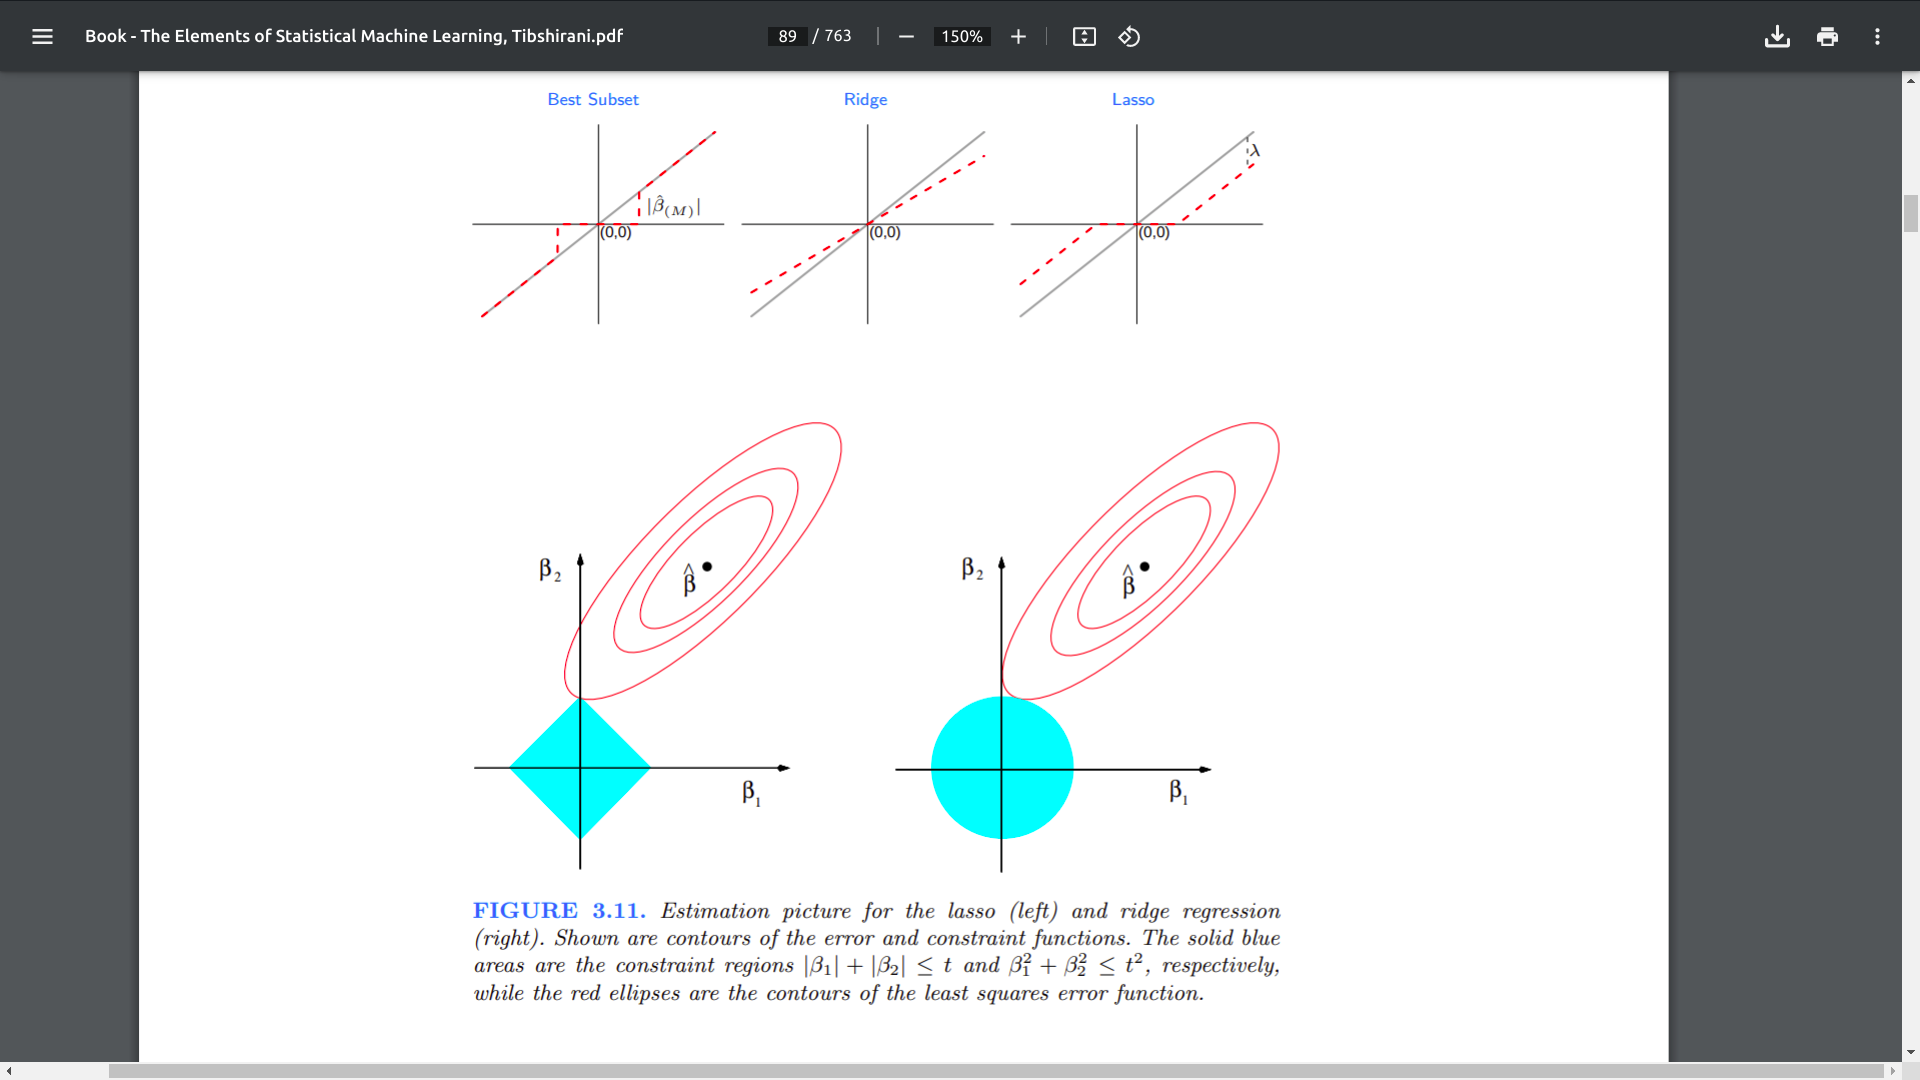
\includegraphics[scale=0.25]{tibshirani_l1_l2.png}
  \caption{Tibshirani Book: Page 71}
  \label{tibs}
\end{figure}

\subsubsection{}
Yes, a closed form for Lasso exists when the features are uncorrelated. \\
We can see this from OLS also, there was a unique solution only when the features were linearly independent. \\
Same way here, if the features are uncorrelated then there is a unique solution which can be found using subgradient methods (Referred to books and search). \\
\begin{figure}[H]
  \centering
  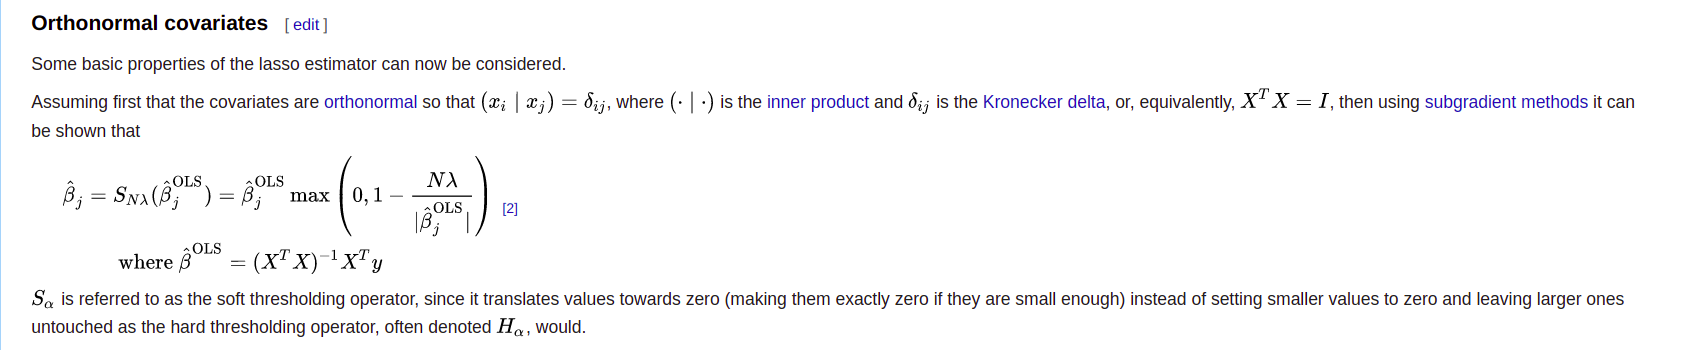
\includegraphics[scale=0.3]{wikipedia_lasso.png}
  \caption{Wikipedia: Lasso (statistics)}
\end{figure}


\newpage
\section{Bias Variance Trade-of}
\subsection{CS 337: Theory}
\subsubsection{}
As discussed in class, Model complexity increases $\implies$ Bias decreases and Variance increases and, Model complexity decreases $\implies$ Bias increases and Variance decreases
\begin{enumerate}
  \item[(a)] Increasing the value of $\lambda$ in lasso regression \\
        $\implies$ Model complexity decreases \\
        $\implies$ Bias increases and Variance decreases
  \item[(b)] Increasing model complexity by adding more features of high degree \\
        $\implies$ Bias decreases and Variance increases
  \item[(c)] Reducing dimension by choosing only those subset of features which are of more importance \\
        $\implies$ Model complexity decreases \\
        $\implies$ Bias increases and Variance decreases
\end{enumerate}

\subsubsection{}
Let the test point be $(x, y = f(x) + \epsilon)$, where $\epsilon \sim \mathcal{N}(0, \sigma^2)$
\begin{equation*}
  \begin{aligned}
    \text{Mean Squared Error} & = \text{E} [ (\hat{f(x)} - y)^2 ]                                                                                                                                      \\
                              & = \text{E} [ \hat{f(x)}^2 + y^2 - 2 \hat{f(x)} y ]                                                                                                                     \\
                              & = \text{E} [(\hat{f(x)} - \overline{\hat{f(x)}})^2] + \overline{\hat{f(x)}}^2 + \text{E} [(y - f(x))^2] + f(x)^2 - 2 \overline{\hat{f(x)}} f(x)                        \\
                              & \bigg[ \text{Using $\text{E} [X^2] = \text{E} [(X - \overline{X})^2] + \overline{X}^2$; $\text{E} [\hat{f(x)}] = \overline{\hat{f(x)}}$; $\text{E} [y] = f(x)$} \bigg] \\
                              & = \text{E} [(\hat{f(x)} - \overline{\hat{f(x)}})^2] + (\overline{\hat{f(x)}} - f(x))^2 + \sigma^2                                                                      \\
                              & = Variance(\hat{f(x)}) + Bias(\hat{f(x)})^2 + \text{irreducible noise variance}
  \end{aligned}
\end{equation*}
Hence proved.

\end{document}
